\documentclass[12pt]{article}

\title{Side Project Summary 2017--2019}
\author{William John Holden}
\date{\today}

\usepackage{amsmath,amsthm}
\usepackage{mathtools}
\usepackage{parskip}
\usepackage{amssymb}
\usepackage[margin=1.0in]{geometry}
\usepackage{minted}
\usepackage[utf8x]{inputenc}
\usepackage[hyphens]{url}
\usepackage[hidelinks]{hyperref}
\usepackage{listings}
\lstset{basicstyle=\ttfamily,columns=flexible,frame=single}
\usepackage{graphicx}

\begin{document}
\maketitle

\begin{abstract}
At 2017--2019 job I worked on several side projects.
I hope that these programs will be useful to others after I leave.
This document catalogs the purpose, capability, and usage of each program.
Only projects that were written directly in support of my job are listed here.
None of these programs require privileged access or installation, although host-based firewalls may interfere with network-aware programs.
\end{abstract}

\section{Connection Map}

\textbf{Language}: Java

\textbf{Location}: \url{https://github.com/wjholden/Connection-Map}

\textbf{Input}: Syslog messages from a Cisco ASA on UDP port 514.

\textbf{Output}: See figure \ref{fig:connection-map}.

\begin{figure}[h]
\centering
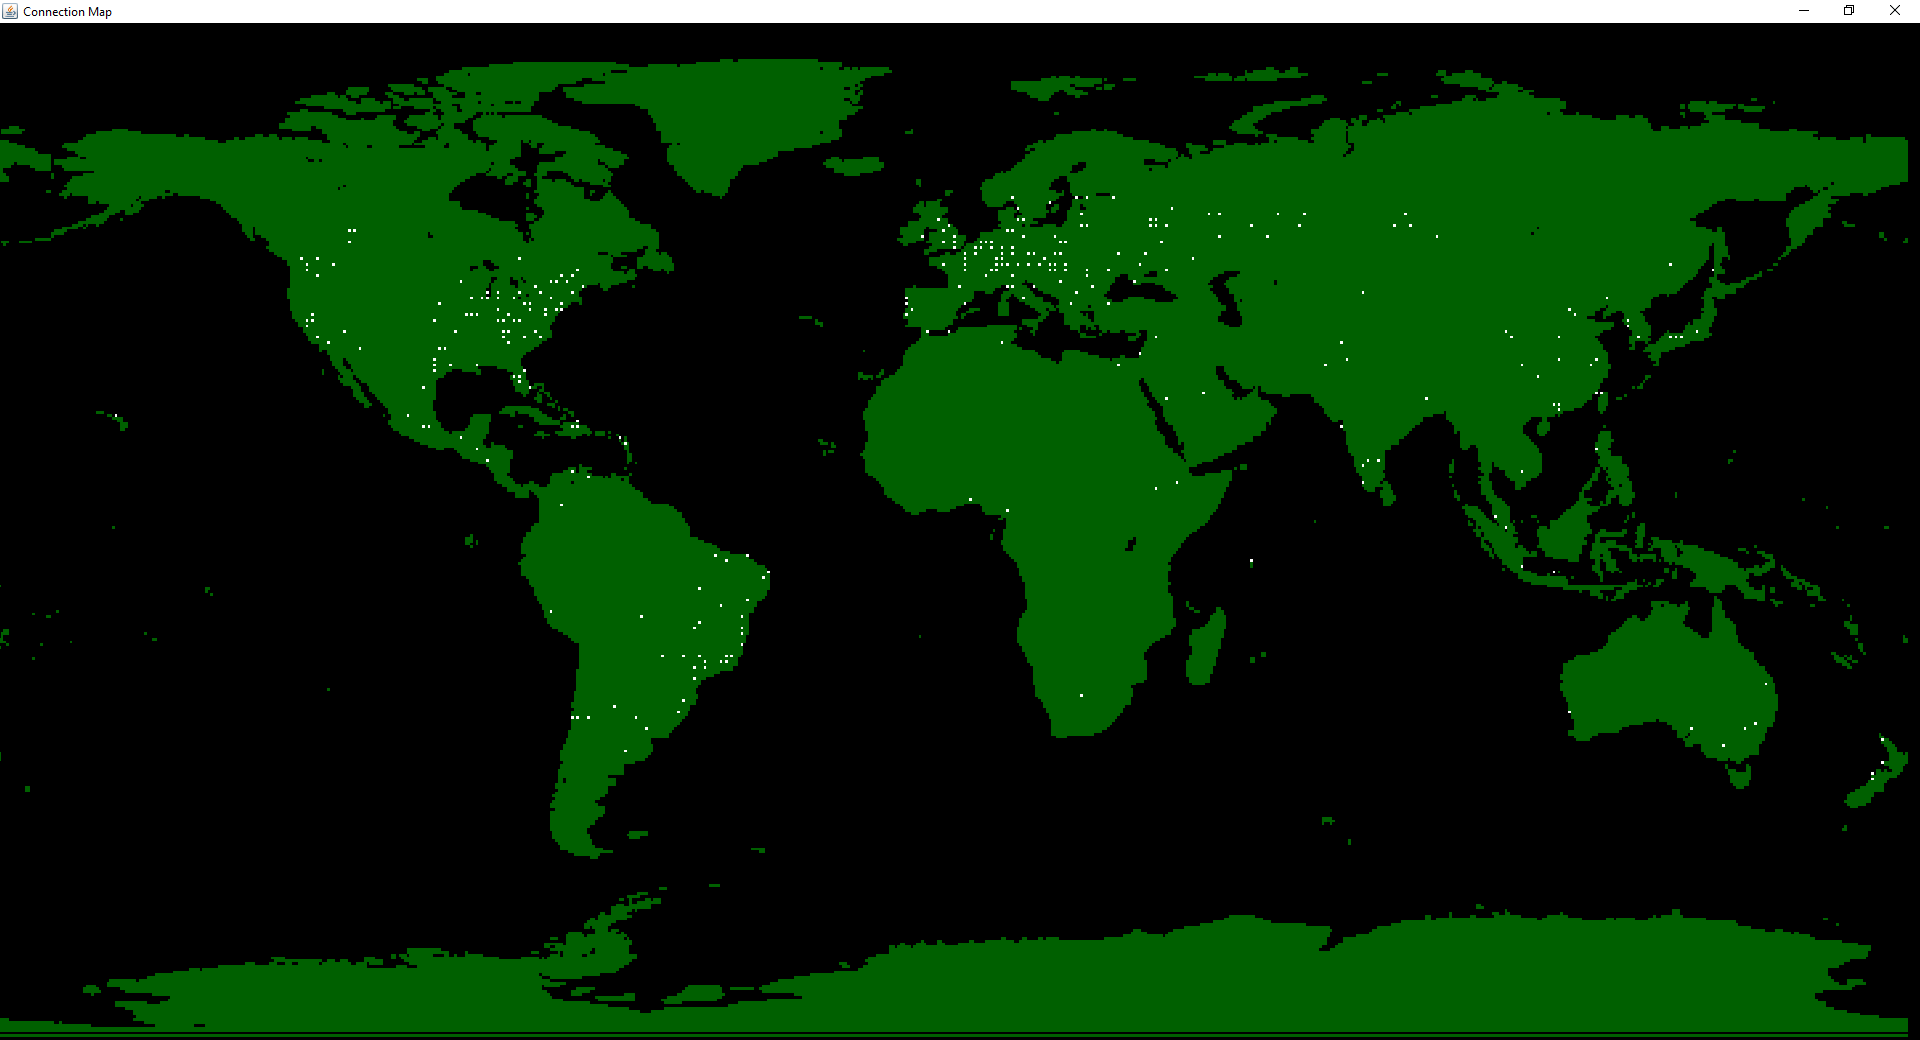
\includegraphics[width=\textwidth]{Connection-Map}
\caption{Connection Map}
\label{fig:connection-map}
\end{figure}

Connection Map is a pure-Java program to visualize network connections through a Cisco ASA firewall on a map. It uses the GeoLite2 ``GeoIP'' database available from \url{https://www.maxmind.com}.

Download the entire project from GitHub with the ``Clone of download'' button and select ``Download ZIP.'' Execute the runnable JAR \texttt{Connection-Map/Connection\_Map.jar}. The \texttt{Connection-Map/lib/} folder must be present and must contain all dependencies.

Press \texttt{h} for a simple help popup listing keyboard shortcuts.

Connection Map passively listens on UDP port 514 for Syslog messages. The program actually opens UDP port 514 as a multicast on the non-standard group \texttt{239.5.1.4}. Connection Map does not allow the operator to select which network interface it will bind to; binding decisions are left to the operating system. Microsoft Windows may bind the socket to an unexpected network interface. Use the command \texttt{netsh interface ipv4 show join} to observe which network interface the socket bound to. Npcap (included with Wireshark) may install a \texttt{Npcap Loopback Adapter} interface and VMware may install a \texttt{VMnet1} interface. These interfaces may have a faster ``speed'' and therefore lower route metric than the physical Ethernet and Wi-Fi interfaces (see \url{https://github.com/nmap/nmap/issues/1605}). If \texttt{netsh interface ipv4 show join} shows that \texttt{239.5.1.4} is joined on the incorrect interface, try disabling the other interface or change its metric (\texttt{Set-NetRoute}).

To configure a Cisco ASA to send Syslog messages to the Connection Map monitoring station, simply input the following commands in global configuration mode:

\begin{lstlisting}
logging enable
logging trap debugging
logging host inside x.x.x.x
\end{lstlisting}

\texttt{x.x.x.x} is either the unicast IP address of the monitoring station or \texttt{239.5.1.4}. The Connection Map program uses regular expressions to find Syslog messages 302013, 302014, 302015, and 302016 (see \url{https://www.cisco.com/c/en/us/td/docs/security/asa/syslog/b_syslog/syslogs3.html}). It assumes the external interface is named \texttt{outside} (case-sensitive). The name of the external interface is not configurable; if the name of the internal interface is not \texttt{outside} then the source code must be modified.

\section{Area Monitor}

Language: Python

\url{https://github.com/wjholden/Area-Monitor}

Input: 

Output: 

\section{lsdb.js}

\section{Node Monitor}

\section{Route Monitor}

\section{Key Chain Generator}

\section{CommSync II Output Interpreter}




\end{document}